\documentclass[fontsize=10pt]{scrartcl}

\usepackage[english]{babel}
\usepackage[utf8]{inputenc}
\usepackage[T1]{fontenc}
\usepackage{lmodern}
\usepackage{amssymb}
\usepackage[autostyle=true]{csquotes}
\usepackage{graphicx}
\usepackage{xcolor}
\usepackage{caption}
\usepackage{url}
\usepackage{float}
\usepackage[hidelinks]{hyperref}
\usepackage{listingsutf8}
\usepackage{fancyheadings}
\usepackage[most]{tcolorbox}
\definecolor{quote-blue}{rgb}{0.95,0.97,0.98}
\newtcolorbox{myquote}{colback=quote-blue,grow to right by=-10mm,grow to left by=-10mm,
    boxrule=0pt,boxsep=0pt,breakable}

\definecolor{rustKeyword}{rgb}{0.54,0.35,0.66}
\definecolor{rustComment}{rgb}{0.56,0.56,0.55}
\definecolor{rustString}{rgb}{0.44,0.55,0}
\definecolor{rustMacro}{rgb}{0.24,0.60,0.62}

\begin{document}
    
    \lstset{
        language=Bash,
        basicstyle=\ttfamily\footnotesize,
        backgroundcolor=\color{white!95!black},
        tabsize=4,
        extendedchars=false,
    }
    
    \lstdefinelanguage{Rust}{
    morekeywords={
        fn,
        use,
    },
    sensitive=true,
    alsoletter={!},
    alsodigit={!},
    morecomment=[l]{//},
    morecomment=[s]{///}{///},
    morestring=[b]"
    }
    
    \lstset{
         language=Rust,
         basicstyle=\ttfamily\footnotesize,
         tabsize=4,
         extendedchars=false,
         keepspaces=true,
         showstringspaces=false,
         breaklines=true,
         commentstyle=\color{rustComment},
         keywordstyle=\color{rustKeyword},
         stringstyle=\color{rustString},
         emph=[1] {
             println!,
         },
         emphstyle=[1]{\color{rustMacro}},
     }
    
    \newcommand{\code}[1]{\lstinline[basicstyle=\ttfamily\color{red!60!black}]|#1|}
    \newcommand{\blank}{\vspace{\baselineskip}}
    \pagestyle{fancy}
    \lhead{\leftmark}
    \rhead{\rightmark}
    \cfoot{\thepage}
    \renewcommand{\headrulewidth}{2pt}
    \renewcommand{\footrulewidth}{1pt}
    
    \begin{titlepage}
\begin{center}

\vspace{1.5cm}
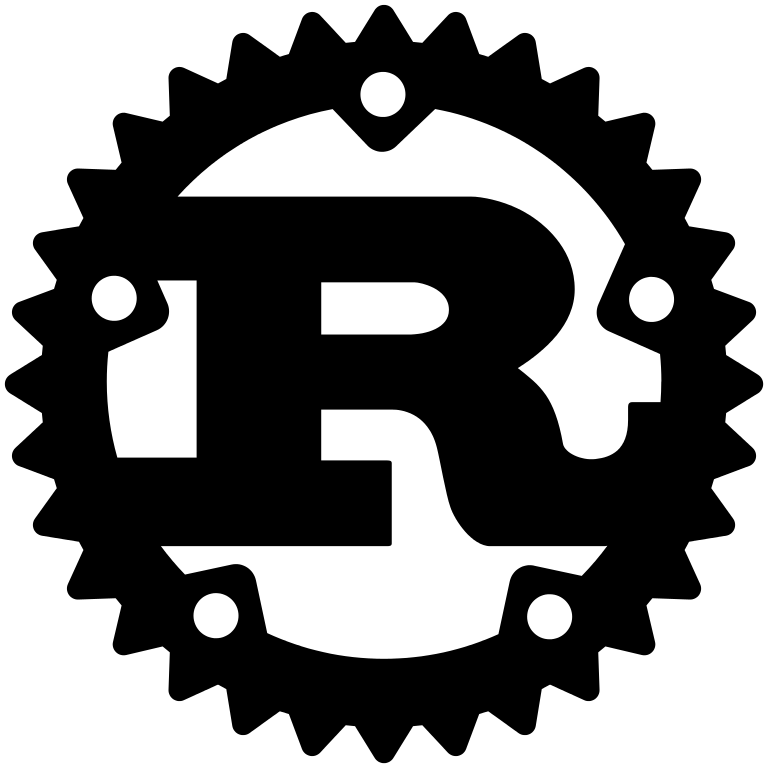
\includegraphics[width=0.5\textwidth]{src/Rust_Logo.png}\\[1cm]

\newcommand{\HRule}{\rule{\linewidth}{0.5mm}}

\HRule\\[1cm]
{\huge \bfseries The Rust Programming Language}\\[1cm]
\HRule\\
\vspace{3cm}

{\large
\textsc{Darth-Revan}\\[0.3cm]
\url{https://github.com/Darth-Revan/rust-lang_Doc-LaTeX}
}
\vfill
{\large \today}


\end{center}
\end{titlepage}

    \pagebreak
    
    \tableofcontents
    \pagebreak

    \pagebreak
    \section{Introduction}
    \label{sec:intro}
    Welcome! This book will teach you about the \href{https://www.rust-lang.org/}{Rust Programming Language}.
Rust is a systems programming language focused on three goals: safety, speed, and concurrency. It maintains 
these goals without having a garbage collector, making it a useful language for a number of use cases other 
languages aren't good at: embedding in other languages, programs with specific space and time requirements, 
and writing low-level code, like device drivers and operating systems. It improves on current languages targeting 
this space by having a number of compile-time safety checks that produce no runtime overhead, while eliminating 
all data races. Rust also aims to achieve 'zero-cost abstractions' even though some of these abstractions feel 
like those of a high-level language. Even then, Rust still allows precise control like a low-level language would.

\blank
\enquote{The Rust Programming Language} is split into chapters. This introduction is the first. After this:

\begin{itemize}
    \item{\nameref{sec:gettingstarted} - Set up your computer for Rust development.}
    \item{\nameref{sec:tutorial} - Learn some Rust with a small project.}
    \item{\nameref{sec:syntax} - Each bit of Rust, broken down into small chunks.}
    \item{\nameref{sec:effective_rust} - Higher-level concepts for writing excellent Rust code.}
    \item{\nameref{sec:nightly_rust} - Cutting-edge features that aren't in stable builds yet.}
    \item{\nameref{sec:glossary} - A reference of terms used in the book.}
    \item{\nameref{sec:bib} - Background on Rust's influences, papers about Rust.}
\end{itemize}

\subsection*{Contributing}

The source files from which this book is generated can be found on
\href{https://github.com/rust-lang/rust/tree/master/src/doc/book}{GitHub}.
    
    \pagebreak
    \section{Getting Started}
    \label{sec:gettingstarted}
    This first chapter of the book will get us going with Rust and its tooling. First, we'll install Rust. Then, the classic 
'Hello World' program. Finally, we'll talk about Cargo, Rust's build system and package manager.

\section{Installing Rust}

The first step to using Rust is to install it. Generally speaking, you'll need an Internet connection to run the commands in 
this section, as we'll be downloading Rust from the internet.

\blank

We'll be showing off a number of commands using a terminal, and those lines all start with \code{\$}. We don't need to type in the 
\code{\$}s, they are there to indicate the start of each command. We'll see many tutorials and examples around the web that follow 
this convention: \code{\$} for commands run as our regular user, and \code{\#} for commands we should be running as an administrator.

\subsection*{Platform support}

The Rust compiler runs on, and compiles to, a great number of platforms, though not all platforms are equally supported. 
Rust's support levels are organized into three tiers, each with a different set of guarantees.

\blank

Platforms are identified by their \enquote{target triple} which is the string to inform the compiler what kind of output should 
be produced. The columns below indicate whether the corresponding component works on the specified platform.

\subsubsection*{Tier 1}

Tier 1 platforms can be thought of as \enquote{guaranteed to build and work}. Specifically they will each satisfy the 
following requirements:

\begin{itemize}
    \item{Automated testing is set up to run tests for the platform.}
    \item{Landing changes to the \code{rust-lang/rust} repository's master branch is gated on tests passing.}
    \item{Official release artifacts are provided for the platform.}
    \item{Documentation for how to use and how to build the platform is available.}
\end{itemize}

\begin{table}[H]
       \centering
       \small
       \begin{tabular}{|l|l|l|l|l|}
           \hline
           \textbf{Target} & \textbf{std} & \textbf{rustc} & \textbf{cargo} & \textbf{notes} \\
           \hline
           \code{x86\_64-pc-windows-msvc} & \checkmark & \checkmark & \checkmark & 64-bit MSVC (Windows 7+) \\
           \code{i686-pc-windows-gnu} & \checkmark & \checkmark & \checkmark & 32-bit MinGW (Windows 7+) \\
           \code{x86\_64-pc-windows-gnu} & \checkmark & \checkmark & \checkmark & 64-bit MinGW (Windows 7+) \\
           \code{i686-apple-darwin} & \checkmark & \checkmark & \checkmark & 32-bit OSX (10.7+, Lion+) \\
           \code{x86\_64-apple-darwin} & \checkmark & \checkmark & \checkmark & 64-bit OSX (10.7+, Lion+) \\
           \code{i686-unkown-linux-gnu} & \checkmark & \checkmark & \checkmark & 32-bit Linux (2.6.18+) \\
           \code{x86\_64-unkown-linux-gnu} & \checkmark & \checkmark & \checkmark & 64-bit Linux (2.6.18+) \\
           \hline
        \end{tabular}
\end{table}

\subsubsection*{Tier 2}

Tier 2 platforms can be thought of as \enquote{guaranteed to build}. Automated tests are not run so it's not guaranteed to produce a 
working build, but platforms often work to quite a good degree and patches are always welcome! Specifically, these platforms are 
required to have each of the following:

\begin{itemize}
    \item{Automated building is set up, but may not be running tests.}
    \item{Landing changes to the \code{rust-lang/rust} repository's master branch is gated on platforms \textbf{building}. Note that this means 
        for some platforms only the standard library is compiled, but for others the full bootstrap is run.}
    \item{Official release artifacts are provided for the platform.}
\end{itemize}

\begin{table}[H]
    \centering
    \small
    \begin{tabular}{|l|l|l|l|l|}
        \hline
        \textbf{Target} & \textbf{std} & \textbf{rustc} & \textbf{cargo} & \textbf{notes} \\
        \hline
        \code{i686-pc-windows-msvc} & \checkmark & \checkmark & \checkmark & 32-bit MSVC (Windows 7+) \\
        \code{x86\_64-unkown-linzux-musl} & \checkmark & & & 64-bit Linux with MUSL \\
        \code{arm-linux-androideabi} & \checkmark & & & ARM Android \\
        \code{arm-unkown-linux-gnueabi} & \checkmark & \checkmark & & ARM Linux (2.6.18+) \\
        \code{arm-unkown-linux-gnueabihf} & \checkmark & \checkmark & & ARM Linux (2.6.18+) \\
        \code{aarch64-unkown-linux-gnu} & \checkmark & & & ARM64 Linux (2.6.18+) \\
        \code{mips-unkown-linux-gnu} & \checkmark & & & MIPS Linux (2.6.18+) \\
        \code{mipsel-unkown-linux-gnu} & \checkmark & & & MIPS (LE) Linux (2.6.18+) \\
        \hline
    \end{tabular}
\end{table}

\subsubsection*{Tier 3}

Tier 3 platforms are those which Rust has support for, but landing changes is not gated on the platform either building or 
passing tests. Working builds for these platforms may be spotty as their reliability is often defined in terms of 
community contributions. Additionally, release artifacts and installers are not provided, but there may be community 
infrastructure producing these in unofficial locations.

\begin{table}[H]
    \centering
    \small
    \begin{tabular}{|l|l|l|l|l|}
        \hline
        \textbf{Target} & \textbf{std} & \textbf{rustc} & \textbf{cargo} & \textbf{notes} \\
        \hline
        \code{i686-linux-android} & \checkmark & & & 32-bit x86 Android \\
        \code{aarch64-linux-android} & \checkmark & & & ARM64 Android \\
        \code{powerpc-unkown-linux-gnu} & \checkmark & & & PowerPC Linux (2.6.18+) \\
        \code{i386-apple-ios} & \checkmark & & & 32-bit x86 iOS \\
        \code{x86\_64-apple-ios} & \checkmark & & & 64-bit x86 iOS \\
        \code{armv7-apple-ios} & \checkmark & & & ARM iOS \\
        \code{armv7s-apple-ios} & \checkmark & & & ARM iOS \\
        \code{aarch64-apple-ios} & \checkmark & & & ARM64 iOS \\
        \code{i686-unkown-freebsd} & \checkmark & \checkmark & & 32-bit FreeBSD \\
        \code{x86\_64-unkown-freebsd} & \checkmark & \checkmark & & 64-bit FreeBSD \\
        \code{x86\_64-unkown-openbsd} & \checkmark & \checkmark & & 64-bit OpenBSD \\
        \code{x86\_64-unkown-netbsd} & \checkmark & \checkmark & & 64-bit NetBSD \\
        \code{x86\_64-unkown-bitrig} & \checkmark & \checkmark & & 64-bit Bitrig \\
        \code{x86\_64-unkown-dragonfly} & \checkmark & \checkmark & & 64-bit DragonFlyBSD \\
        \code{x86\_64-rumprun-netbsd} & \checkmark & & & 64-bit NetBDS Rump Kernel \\
        \code{i686-pc-windows-msvc (XP)} & \checkmark & & & Windows XP support \\
        \code{x86\_64-pc-windows-msvc (XP)} & \checkmark & & & Windows XP support \\
        \hline
    \end{tabular}
\end{table}

Note that this table can be expanded over time, this isn't the exhaustive set of tier 3 platforms that will ever be!

\subsection*{Installing on Linux or Mac}

If we're on Linux or a Mac, all we need to do is open a terminal and type this:

\begin{verbatim}
$ curl -sSf https://static.rust-lang.org/rustup.sh | sh
\end{verbatim}

This will download a script, and stat the installation. If it all goes well, you'll see this appear:

\begin{verbatim}
Welcome to Rust.

This script will download the Rust compiler and its package manager, 
Cargo, and install them to /usr/local. You may install elsewhere by 
running this script with the --prefix=<path> option.

The installer will run under 'sudo' and may ask you for your password. 
If you do not want the script to run 'sudo' then pass it the 
--disable-sudo flag.

You may uninstall later by running /usr/local/lib/rustlib/uninstall.sh,
or by running this script again with the --uninstall flag.

Continue? (y/N)
\end{verbatim}

From here, press \code{y} for 'yes', and then follow the rest of the prompts.

\subsection*{Installing on Windows}

If you're on Windows, please download the appropriate \href{https://www.rust-lang.org/install.html}{installer}.

\subsection*{Uninstalling}

Uninstalling Rust is as easy as installing it. On Linux or Mac, run the uninstall script:

\begin{verbatim}
$ sudo /usr/local/lib/rustlib/uninstall.sh
\end{verbatim}

If we used the Windows installer, we can re-run the \code{.msi} and it will give us an uninstall option.

\subsection*{Troubleshooting}

If we've got Rust installed, we can open up a shell, and type this:

\begin{verbatim}
$ rustc --version
\end{verbatim}

You should see the version number, commit hash, and commit date.

\blank

If you do, Rust has been installed successfully! Congrats!

\blank

If you don't and you're on Windows, check that Rust is in your \%PATH\% system variable. If it isn't, run the installer again, 
select \enquote{Change} on the \enquote{Change, repair, or remove installation} page and ensure \enquote{Add to PATH} is installed 
on the local hard drive.

\blank

If not, there are a number of places where we can get help. The easiest is the 
\href{irc://irc.mozilla.org/\#rust}{\#rust IRC channel on irc.mozilla.org}, which we can access through
\href{http://chat.mibbit.com/?server=irc.mozilla.org&channel=\%23rust}{Mibbit}. Click that link, and we'll be chatting with other 
Rustaceans (a silly nickname we call ourselves) who can help us out. Other great resources include 
\href{https://users.rust-lang.org/}{the user's forum}, and \href{http://stackoverflow.com/questions/tagged/rust}{Stack Overflow}.

\blank

This installer also installs a copy of the documentation locally, so we can read it offline. On UNIX systems, \code{/usr/local/share/doc/rust} 
is the location. On Windows, it's in a \code{share/doc directory}, inside the directory to which Rust was installed.

\section{Hello, World!}

Now that you have Rust installed, we'll help you write your first Rust program. It's traditional when learning a new language 
to write a little program to print the text \enquote{Hello, world!} to the screen, and in this section, we'll follow that 
tradition.

\blank

The nice thing about starting with such a simple program is that you can quickly verify that your compiler is installed, 
and that it's working properly. Printing information to the screen is also a pretty common thing to do, so practicing it 
early on is good.

\begin{myquote}
    Note: This book assumes basic familiarity with the command line. Rust itself makes no specific demands about your editing,
    tooling, or where your code lives, so if you prefer an IDE to the command line, that's an option. You may want to check out
    SolidOak, which was built specifically with Rust in mind. There are a number of extensions in development by the community, 
    and the Rust team ships plugins for various editors. Configuring your editor or IDE is out of the scope of this tutorial, so
    check the documentation for your specific setup.
\end{myquote}

\subsection*{Creating a Project File}

First, make a file to put your Rust code in. Rust doesn't care where your code lives, but for this book, I suggest making a 
\emph{projects} directory in your home directory, and keeping all your projects there. Open a terminal and enter the following 
commands to make a directory for this particular project:

\begin{verbatim}
$ mkdir ~/projects
$ cd ~/projects
$ mkdir hello_world
$ cd hello_world
\end{verbatim}

\begin{myquote}
Note: If you're on Windows and not using PowerShell, the ~ may not work. Consult the documentation for your shell for more details.
\end{myquote}

\subsection*{Writing and Running a Rust Program}

Next, make a new source file and call it \emph{main.rs}. Rust files always end in a \emph{.rs} extension. If you're using more 
than one word in your filename, use an underscore to separate them; for example, you'd use \emph{hello\_world.rs} rather than 
\emph{helloworld.rs}.

\blank

Now open the main.rs file you just created, and type the following code:

\begin{rustc}
fn main() {
    println!("Hello, world!");
}
\end{rustc}

Save the file, and go back to your terminal window. On Linux or OSX, enter the following commands:

\begin{verbatim}
$ rustc main.rs
$ ./main
Hello, world!
\end{verbatim}

In Windows, replace \code{main} with \code{main.exe}. Regardless of your operating system, you should see the string 
\code{Hello, world!} print to the terminal. If you did, then congratulations! You've officially written a Rust program. 
That makes you a Rust programmer! Welcome.

\subsection*{Anatomy of a Rust Program}

Now, let's go over what just happened in your \enquote{Hello, world!} program in detail. Here's the first piece of the puzzle:

\begin{rustc}
fn main() {
    
}
\end{rustc}

These lines define a \emph{function} in Rust. The \code{main} function is special: it's the beginning of every Rust program. The 
first line says, \enquote{I'm declaring a function named \code{main} that takes no arguments and returns nothing.} If there were 
arguments, they would go inside the parentheses (\code{(} and \code{)}), and because we aren't returning anything from this function, 
we can omit the return type entirely.

\blank

Also note that the function body is wrapped in curly braces (\code{\{} and \code{\}}). Rust requires these around all function
bodies. It's considered good style to put the opening curly brace on the same line as the function declaration, with one space 
in between.

\blank

Inside the \code{main()} function:

\begin{rustc}
println!("Hello, world!");
\end{rustc}

This line does all of the work in this little program: it prints text to the screen. There are a number of details that are important 
here. The first is that it's indented with four spaces, not tabs.

\blank

% TODO make macro a hyperref to the macro section
The second important part is the \code{println!()} line. This is calling a Rust \emph{macro}, which is how metaprogramming is done 
in Rust. If it were calling a function instead, it would look like this: \code{println()} (without the !). We'll discuss Rust macros 
in more detail later, but for now you only need to know that when you see a \code{!} that means that you're calling a macro 
instead of a normal function.

\blank

% TODO make statically allocated string a hyperref to the section about the stack and heap
Next is \code{"Hello, world!"} which is a \emph{string}. Strings are a surprisingly complicated topic in a systems programming 
language, and this is a statically allocated string. We pass this string as an argument to \code{println!}, which prints the 
string to the screen. Easy enough!

\blank

The line ends with a semicolon (\code{;}). Rust is an \nameref{sec:gloss_expressionorientedlang}, which means that most things are 
expressions, rather than statements. The \code{;} indicates that this expression is over, and the next one is ready 
to begin. Most lines of Rust code end with a \code{;}.

\subsection*{Compiling and Running are Separate Steps}

In \enquote{Writing and Running a Rust Program}, we showed you how to run a newly created program. We'll break that process 
down and examine each step now.

\blank

Before running a Rust program, you have to compile it. You can use the Rust compiler by entering the 
\code{rustc} command and passing it the name of your source file, like this:

\begin{verbatim}
$ rustc main.rs
\end{verbatim}

If you come from a C or C++ background, you'll notice that this is similar to \code{gcc} or \code{clang}. After 
compiling successfully, Rust should output a binary executable, which you can see on Linux or OSX by entering the 
\code{ls} command in your shell as follows:

\begin{verbatim}
$ ls
main main.rs 
\end{verbatim}

On Windows, you'd enter:

\begin{verbatim}
$ dir
main.exe main.rs  
\end{verbatim}

This shows we have two files: the source code, with an \code{.rs} extension, and the executable (\code{main.exe} on Windows, 
\code{main} everywhere else). All that's left to do from here is run the \code{main} or \code{main.exe} file, like this:

\begin{verbatim}
$./main  # or main.exe on Windows  
\end{verbatim}

If \emph{main.rs} were your \enquote{Hello, world!} program, this would print \code{Hello, world!} to your terminal.

\blank

If you come from a dynamic language like Ruby, Python, or JavaScript, you may not be used to compiling and running a program 
being separate steps. Rust is an \emph{ahead-of-time compiled} language, which means that you can compile a program, give it 
to someone else, and they can run it even without Rust installed. If you give someone a \code{.rb} or \code{.py} or \code{.js} 
file, on the other hand, they need to have a Ruby, Python, or JavaScript implementation installed (respectively), but you only 
need one command to both compile and run your program. Everything is a tradeoff in language design.

\blank

Just compiling with \code{rustc} is fine for simple programs, but as your project grows, you'll want to be able to manage all 
of the options your project has, and make it easy to share your code with other people and projects. Next, I'll introduce you 
to a tool called Cargo, which will help you write real-world Rust programs.

\section{Hello, Cargo!}
\label{sec:gettingstarted_helloCargo}

Cargo is Rust's build system and package manager, and Rustaceans use Cargo to manage their Rust projects. Cargo manages 
three things: building your code, downloading the libraries your code depends on, and building those libraries. We call 
libraries your code needs 'dependencies' since your code depends on them.

\blank

The simplest Rust programs don't have any dependencies, so right now, you'd only use the first part of its functionality. 
As you write more complex Rust programs, you'll want to add dependencies, and if you start off using Cargo, that will be 
a lot easier to do.

\blank

As the vast, vast majority of Rust projects use Cargo, we will assume that you're using it for the rest of the book. 
Cargo comes installed with Rust itself, if you used the official installers. If you installed Rust through some other 
means, you can check if you have Cargo installed by typing:

\begin{verbatim}
$ cargo --version
\end{verbatim}

into a terminal. If you see a version number, great! If you see an error like '\code{command not found}', then you should look 
at the documentation for the system in which you installed Rust, to determine if Cargo is separate.

\subsection*{Converting to Cargo}

Let's convert the Hello World program to Cargo. To Cargo-fy a project, you need to do three things:

\begin{enumerate}
    \item{Put your source file in the right directory.}
    \item{Get rid of the old executable (\code{main.exe} on Windows, \code{main} everywhere else) and make a new one.}
    \item{Make a Cargo configuration file.}
\end{enumerate}

Let's get started!

\subsubsection*{Creating a new Executable and Source Directory}

First, go back to your terminal, move to your \emph{hello\_world} directory, and enter the following commands:

\begin{verbatim}
$ mkdir src
$ mv main.rs src/main.rs
$ rm main  # or 'del main.exe' on Windows 
\end{verbatim}

Cargo expects your source files to live inside a \emph{src} directory, so do that first. This leaves the top-level 
project directory (in this case, \emph{hello\_world}) for READMEs, license information, and anything else not related 
to your code. In this way, using Cargo helps you keep your projects nice and tidy. There's a place for everything, 
and everything is in its place.

\blank

Now, copy \emph{main.rs} to the \emph{src} directory, and delete the compiled file you created with \code{rustc}. As usual, 
replace \code{main} with \code{main.exe} if you're on Windows.

\blank

This example retains \code{main.rs} as the source filename because it's creating an executable. If you wanted to make a 
library instead, you'd name the file \code{lib.rs}. This convention is used by Cargo to successfully compile your projects, 
but it can be overridden if you wish.

\subsubsection*{Creating a Configuration File}

Next, create a new file inside your \emph{hello\_world} directory, and call it \code{Cargo.toml}.

\blank

Make sure to capitalize the \code{C} in \emph{Cargo.toml}, or Cargo won't know what to do with the configuration file.

\blank

This file is in the \href{https://github.com/toml-lang/toml}{TOML} (Tom's Obvious, Minimal Language) format. TOML is similar 
to INI, but has some extra goodies, and is used as Cargo's configuration format.

\blank

Inside this file, type the following information:

\begin{verbatim}
[package]

name = "hello_world"
version = "0.0.1"
authors = [ "Your name <you@example.com>" ] 
\end{verbatim}

The first line, \code{[package]}, indicates that the following statements are configuring a package. As we add more information 
to this file, we'll add other sections, but for now, we only have the package configuration.

\blank

The other three lines set the three bits of configuration that Cargo needs to know to compile your program: its name, what 
version it is, and who wrote it.

\blank

Once you've added this information to the \emph{Cargo.toml} file, save it to finish creating the configuration file.

\subsection*{Building and Running a Cargo Project}

With your \emph{Cargo.toml} file in place in your project's root directory, you should be ready to build and run your 
Hello World program! To do so, enter the following commands:

\begin{verbatim}
$ cargo build
   Compiling hello_world v0.0.1 (file:///home/yourname/projects/hello_world)
$ ./target/debug/hello_world
Hello, world! 
\end{verbatim}

Bam! If all goes well, \code{Hello, world!} should print to the terminal once more.

\blank

You just built a project with \code{cargo build} and ran it with \code{./target/debug/hello\_world}, but you can actually do 
both in one step with \code{cargo} run as follows:

\begin{verbatim}
$ cargo run
     Running `target/debug/hello_world`
Hello, world!  
\end{verbatim}

Notice that this example didn't re-build the project. Cargo figured out that the file hasn't changed, and so it just 
ran the binary. If you'd modified your source code, Cargo would have rebuilt the project before running it, and you 
would have seen something like this:

\begin{verbatim}
$ cargo run
   Compiling hello_world v0.0.1 (file:///home/yourname/projects/hello_world)
     Running `target/debug/hello_world`
Hello, world!  
\end{verbatim}

Cargo checks to see if any of your project's files have been modified, and only rebuilds your project if they've changed since 
the last time you built it.

\blank

With simple projects, Cargo doesn't bring a whole lot over just using \code{rustc}, but it will become useful in future. This 
is especially true when you start using crates; these are synonymous with a 'library' or 'package' in other programming languages. 
For complex projects composed of multiple crates, it's much easier to let Cargo coordinate the build. Using Cargo, you can run 
\code{cargo build}, and it should work the right way.

\subsubsection*{Building for Release}

When your project is finally ready for release, you can use \code{cargo build --release} to compile your project with optimizations. 
These optimizations make your Rust code run faster, but turning them on makes your program take longer to compile. This is why 
there are two different profiles, one for development, and one for building the final program you'll give to a user.

\blank

Running this command also causes Cargo to create a new file called \emph{Cargo.lock}, which looks like this:

\begin{verbatim}
[root]
name = "hello_world"
version = "0.0.1"
\end{verbatim}

Cargo uses the \emph{Cargo.lock} file to keep track of dependencies in your application. This is the Hello World project's 
\emph{Cargo.lock} file. This project doesn't have dependencies, so the file is a bit sparse. Realistically, you won't ever 
need to touch this file yourself; just let Cargo handle it.

\blank

That's it! If you've been following along, you should have successfully built \code{hello\_world} with Cargo.

\blank

Even though the project is simple, it now uses much of the real tooling you'll use for the rest of your Rust career. 
In fact, you can expect to start virtually all Rust projects with some variation on the following commands:

\begin{verbatim}
$ git clone someurl.com/foo
$ cd foo
$ cargo build 
\end{verbatim}

\subsection*{Making a new Cargo Project the Easy Way}

You don't have to go through that previous process every time you want to start a new project! Cargo can quickly make a 
bare-bones project directory that you can start developing in right away.

\blank

To start a new project with Cargo, enter \code{cargo new} at the command line:

\begin{verbatim}
$ cargo new hello_world --bin
\end{verbatim}

This command passes \code{--bin} because the goal is to get straight to making an executable application, as opposed to a 
library. Executables are often called binaries (as in \code{/usr/bin}, if you're on a Unix system).

\blank

Cargo has generated two files and one directory for us: a \code{Cargo.toml} and a \emph{src} directory with a \emph{main.rs}
file inside. These should look familliar, they're exactly what we created by hand, above.

\blank

This output is all you need to get started. First, open \code{Cargo.toml}. It should look something like this:

\begin{verbatim}
[package]

name = "hello_world"
version = "0.1.0"
authors = ["Your Name <you@example.com>"]  
\end{verbatim}

Cargo has populated \emph{Cargo.toml} with reasonable defaults based on the arguments you gave it and your \code{git}
global configuration. You may notice that Cargo has also initialized the \code{hello\_world} directory as a \code{git} 
repository.

\blank

Here's what should be in \code{src/main.rs}:

\begin{rustc}
fn main() {
    println!("Hello, world!");
}
\end{rustc}

Cargo has generated a \enquote{Hello World!} for you, and you're ready to start coding!

\begin{myquote}
Note: If you want to look at Cargo in more detail, check out the official \href{http://doc.crates.io/guide.html}{Cargo guide}, 
which covers all of its features.
\end{myquote}

\section{Closing Thoughts}

This chapter covered the basics that will serve you well through the rest of this book, and the rest of your time with Rust. 
Now that you've got the tools down, we'll cover more about the Rust language itself.

\blank

% TODO make syntax and semantics a hyperref
You have two options: Dive into a project with 'Learn Rust', or start from the bottom and work your way up with 
'Syntax and Semantics'. More experienced systems programmers will probably prefer 'Learn Rust', while those from 
dynamic backgrounds may enjoy either. Different people learn differently! Choose whatever's right for you.

    
    \pagebreak
    \section{Tutorial: Guessing Game}
    \label{sec:tutorial}
    
    \pagebreak
    \section{Syntax and Semantics}
    \label{sec:syntax}
    
    \pagebreak
    \section{Effective Rust}
    \label{sec:effective_rust}
    
    \pagebreak
    \section{Nightly Rust}
    \label{sec:nightly_rust}
    
    \pagebreak
    \section{Glossary}
    \label{sec:glossary}
    
    \pagebreak
    \section{Syntax Index}
    \label{sec:syntax_index}
    
    \pagebreak
    \section{Bibliography}
    \label{sec:bib}
    
\end{document}
